\section{Kinect SDK}\label{SDK}
%(Essenz auf der praktischen Anwendung des SKDs -> Methoden, Funktionen)
%
%
%	History des SDKs? -> kinect for windows sdk programming guide%
%
%	Wichtigste Methoden: 
%		C#, u.a. auch wegen Nao
%		Bibliothekseinbindung
%			using Microsoft.Kinect
%			Assemblyverweis
%		Connect/Disconnect -> Tiefenstream & Skeletonstream aktivieren
%		Eventhandling
%
%	Tools die mir zur Verfügung stehen zum Debugging
%		Kinect Studio
%		Samples/Templates
%
%
%Rauminformationen für Software
%Vorteil: Günstig, leicht zu entwickeln, da SDK vorhanden

%Da das Produkt Xbox Kinect bereits vor einigen Jahren auf den Markt kam, hatten die Entwickler Zeit, um ein SDK zu entwickeln, was alle wichtigen Programmfunktionen bereits enthält. Dies macht es einem Entwickler relativ leicht eine Anwendung zu erstellen, die bestimmte Kinect-Funktionen bereitstellt. 
	
\subsection{Timeline}
Nach dem Erscheinen der Kinect - Kamera war diese auch schnell in Entwicklerkreisen gefragt. Microsoft selbst gefiel dies zunächst nicht, denn der Konzern befürchtete, dass Cheater (engl.: Betrüger) sich an ihren Spielen zu schaffen machen würden und somit den Spielspaß mindern würden. So veröffentlichte Microsoft selbst zunächst kein SDK. Die Open Source Gemeinde jedoch erkannte das Potential des Produktes schnell und entwickelte eine Schnittstelle zu \textit{OpenNI}, einem Framework, das die Auswertung von 3D-Sensordaten verschiedenster Hersteller unterstützt. Dieses Framework bietet somit durch seine Plattformunabhängigkeit die Möglichkeit unterschiedliche Betriebssysteme mit unterschiedlichen 3D-Sensoren zu kombinieren.\cite{webb2012beginning}
Microsoft zog nach und veröffentlichte am 17. Juni 2011 die freie Beta Version des Microsoft SDK. Somit hatte nun jeder Entwickler freien Zugang zu allen Kinectfunktionen, die auch von Microsoft selbst bisher genutzt wurden. Einer der Vorteile des Kinect SDK besteht darin, dass die Skelett-Erkennung (Siehe Kapitel \ref{Software} \nameref{Software}) ohne initiale Pose möglich ist, was im Gegensatz zum OpenNI-Framework steht. \cite{webb2012beginning} Da für dieses Projekt die Plattformunabhängigkeit nicht relevant ist, jedoch aber die Skeletterkennung, fiel die Entscheidung auf das Microsoft Kinect SDK.

%
% WPF Grundlagen erklaeren!!!
%	Trennung Visuelle Beschreibung und Programm .cs, .xaml	
%	Thread Konzept erlaeuter, das Problem darstellte, Security Dispatcher fuer WindowFrame
%
%\todo{Etwas ueber WPF schreiben)

\subsection{Grundfunktionen}
Anhand des folgenden Listings sollen die grundlegenden Funktion der vorhandenen Bibliotheken und deren Verwendungsweisen verdeutlicht werden:

\lstinputlisting
    [caption={Initialisierung des Kinect Sensors \cite{pdf:maccormick}}
       \label{lst:kinect_sdk},
       captionpos=b]
 {Listings/Kinect_Sample.cs}
\noindent
Zuerst muss die Kinect-Bibliothek in C\# eingebunden werden (Zeile 1). Danach kann ein Sensorobjekt instanziiert werden. Dieses erreicht man über ein Array, da gleichzeitig mehrere Kinect-Systeme per USB angeschlossen und verwendet werden könnten (Zeile 7). Für dieses Projekt wird jedoch nur eine Hardware benötigt und somit handelt es sich immer um das Element mit dem Index 0. Im Anschluss daran wird der Tiefenstream des Sensors aktiviert (Zeile 10) und ein \textit{DepthFrameReady} Event registriert und mit der Methode sensor\_DepthFrameReady (Ab Zeile 21) verknüpft. Diese Methode wird somit bei jeder Aktualisierung der Tiefenwerte aufgerufen und liefert die aktuellen Werte, die in einem Short-Array gespeichert werden. \\ \\
\textbf{Anmerkung}\\
In diesem Listing fehlt die Freigabe von Kinect nach Terminierung der Applikation. Aus diesem Grund
registiert man einen WindowClosing-Listener, der die jeweiligen aktivierten Funktionen richtig deaktiviert. Dies ist nicht zwingend nötig, aber wird das Programm beendet, bleibt der IR-Emitter aktiviert und es kann zu Komplikationen führen, wenn das Programm erneut auf die Funktionen zugreifen möchte.

\subsection{Skelettfunktionen}
Zur Nutzung des Skelett-Trackings muss eine Anwendung ähnlich dem obigen Listing initialisiert werden.
In diesem Fall aktiviert man den Skeletonstream mit \textit{sensor.SkeletonStream.Enable()} und registriert wie oben auch ein Event. In diesem Fall ein \textit{SkeletonFrameReady}-Event und verknüpft dieses wie oben mit einer Methode. Folgender Codeausschnitt zeigt die Verwendung des Skeletonstream innerhalb dieses Projektes in C\#.\\

\lstinputlisting
    [caption={Verwendung des Skeleton-Streams}
       \label{lst:kinect_skeleton_stream},
       captionpos=b]
{Listings/Kinect_Skeleton.cs}

\noindent
Erkennt die Kinect einen Spieler im Sichtfeld, wird ein SkeletonFrameReady-Event erzeugt und die registrierte Methode aufgerufen. Da in diesem Projekt der RGB-Stream und der Skeleton-Stream gleichzeitig benötigt werden, gibt es auch die Möglichkeit ein \textit{AllFramesReady}-Event zu registrieren, dass Informationen aller Streams beinhaltet. Im obigen Listing ist ein Auszug aus der Methode \textit{runtime\_AllFramesReady}. Diese erhält über die Methode \textit{OpenSkeletonFrame} das Skelettobjekt. Danach kann das Objekt entsprechend verwendet werden. Falls ein neues Skelett vorhanden ist, wird dieses in einem Array vom Typ \textbf{Skeleton} gespeichert (Zeile 10). Da innerhalb dieses Projektes jedoch nur ein Benutzer relevant ist, wird zur Weiterverarbeitung nur das aktive Skelett des ersten Spielers verwendet. Existiert ein neues Skelett, wird dieses an den Handler übergeben, der die Schnittstelle zur weiteren Verarbeitung des Skeletts darstellt (Zeile 24). Auf die genaue Funktion dieses Handlers wird im Kapitel \myref{k:Architektur} näher eingegangen.

%\todo{Screenshot Skelett}
%
% Screenshot eines Skeletts 
%

\subsection{Kinect Studio}
Das Kinect-SDK stellt einem Entwickler nach der Installation nützliche Dinge bereit, wie eine Bibliothek mit verschiedenen Templates, die beschreiben, wie die Funktionen der Kinect aus Microsoft Sicht verwendet werden. Zusätzlich zu den Templates wird mit dem SDK auch das Kinect Studio mitgeliefert. Diese Anwendung ist für die Entwicklung von Kinect Applikationen sehr nützlich, da man hier wie bei einem Videoschnittprogramm Sequenzen aufnehmen kann, die RGB und Tiefendaten enthalten. Zudem erkennt Kienct Studio aktive Kinect-Applikationen und kann sich zu diesen verbinden. Somit können Bewegungen aufgenommen werden und in der entwickelten Anwendung \textit{abgespielt} werden, ohne diese immer vor der Kinect ausführen zu müssen.
%\todo{Screenshot Kinect-Studio}
\begin{figure}[H]						
	\centering							
	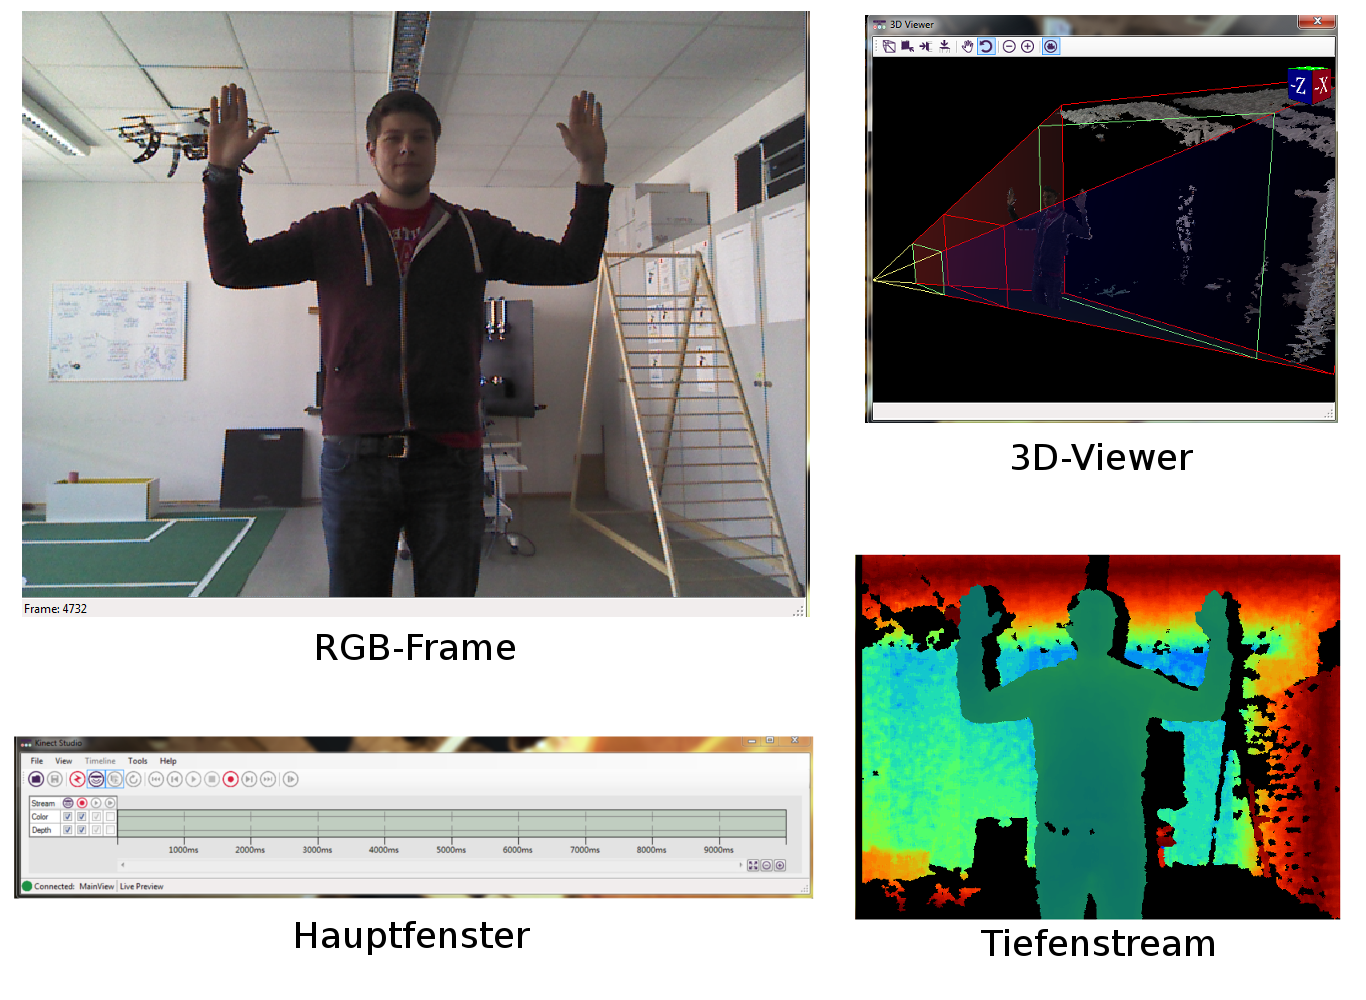
\includegraphics[scale=0.4]{Bilder/Kinect_Studio.png}			
	\caption{Kinect Studio}						
	\label{f:kinect_studio}						
\end{figure}
\textbf{Anmerkung}\\
Das Verbinden funktioniert jedoch nur, wenn Kinect per USB aktuell angeschlossen ist. Deshalb benötigt man zwingend ein Kinect-Modul, um seine Anwendung testen zu können.